%for a more compact document, add the option openany to avoid
%starting all chapters on odd numbered pages
\documentclass[12pt]{cmuthesis}

% This is a template for a CMU thesis.  It is 18 pages without any content :-)
% The source for this is pulled from a variety of sources and people.
% Here's a partial list of people who may or may have not contributed:
%
%        bnoble   = Brian Noble
%        caruana  = Rich Caruana
%        colohan  = Chris Colohan
%        comar    = Cyrus Omar
%        jab      = Justin Boyan
%        josullvn = Joseph O'Sullivan
%        jrs      = Jonathan Shewchuk
%        kosak    = Corey Kosak
%        mjz      = Matt Zekauskas (mattz@cs)
%        pdinda   = Peter Dinda
%        pfr      = Patrick Riley
%        dkoes = David Koes (me)

% My main contribution is putting everything into a single class files and small
% template since I prefer this to some complicated sprawling directory tree with
% makefiles.

% some useful packages
\usepackage{times}
\usepackage{fullpage}
\usepackage{graphicx}
\usepackage{amsmath}
\usepackage[numbers,sort]{natbib}
\usepackage[backref,pageanchor=true,plainpages=false, pdfpagelabels, bookmarks,bookmarksnumbered,
%pdfborder=0 0 0,  %removes outlines around hyper links in online display
]{hyperref}
\usepackage{subfigure}

%%%
\usepackage{url}
%%%

% Approximately 1" margins, more space on binding side
%\usepackage[letterpaper,twoside,vscale=.8,hscale=.75,nomarginpar]{geometry}
%for general printing (not binding)
\usepackage[letterpaper,twoside,vscale=.8,hscale=.75,nomarginpar,hmarginratio=1:1]{geometry}

% Provides a draft mark at the top of the document. 
\draftstamp{\today}{DRAFT}

\begin {document} 
\frontmatter

%initialize page style, so contents come out right (see bot) -mjz
\pagestyle{empty}

\title{ %% {\it \huge Thesis Proposal}\\
{\bf Awesome Work in Computer Science}}
\author{Me}
\date{January 3006}
\Year{3006}
\trnumber{}

\committee{
Nearly Divine Personage, Chair \\
Someone else \\
Yet another person \\
Someone from a strange and faraway land
}

\support{}
\disclaimer{}

% copyright notice generated automatically from Year and author.
% permission added if \permission{} given.

\keywords{Stuff, More Stuff}

\maketitle

\begin{dedication}
For my dog
\end{dedication}

\pagestyle{plain} % for toc, was empty

%% Obviously, it's probably a good idea to break the various sections of your thesis
%% into different files and input them into this file...

\begin{abstract}
A short summary.
\end{abstract}

\begin{acknowledgments}
My advisor is cool.
\end{acknowledgments}


\newcommand \figureone{
\begin{figure}[h]
\centering
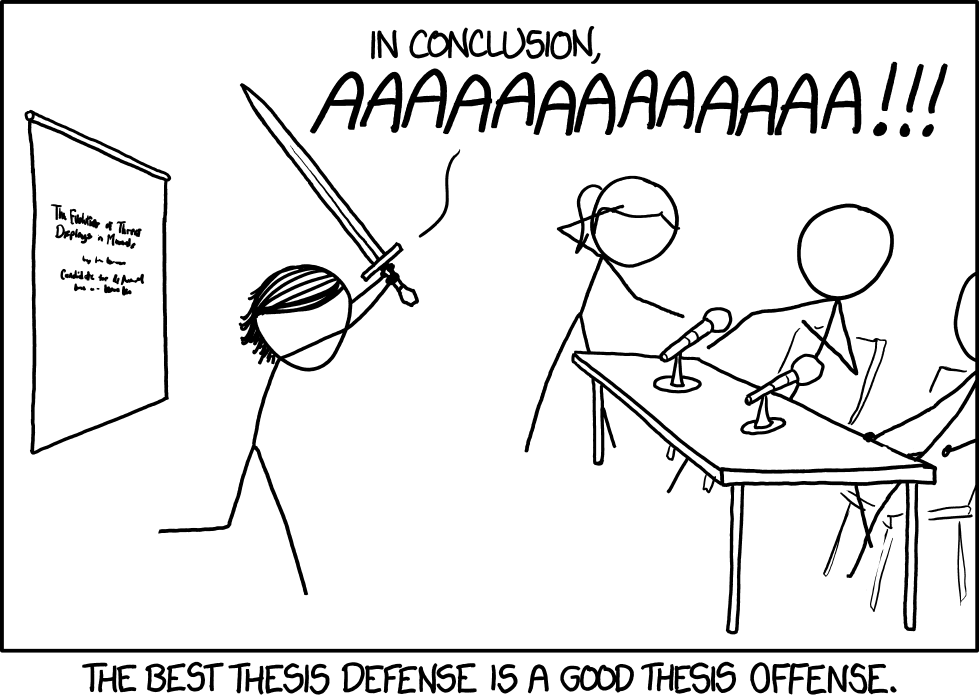
\includegraphics[width=0.99\linewidth]{fig/fig1.png}
\caption{An example figure. Source  \url{https://xkcd.com/1403/}}\label{fig1}
\end{figure}
}

\newcommand \tableone{
\begin{table}[t]
\centering
\begin{tabular}{@{}lrrrrrrrrrr@{}}
\toprule
 & \textbf{1} & \textbf{2} & \textbf{3} & \textbf{4} & \textbf{5} & \textbf{6} & \textbf{7} & \textbf{8} & \textbf{9} & \textbf{10} \\ \midrule
\textbf{1} & 0 & $\frac{1}{2}$ & 4 & 5 & 6 & 7 & 8 & 9 & 10 & 9 \\
\textbf{2} & $\frac{1}{2}$ & 8 & 5 & 6 & 12 & 14 & 12 & 18 & 19 & 22 \\
\textbf{3} & 4 & 5 & 10 & 16 & 13 & 12 & 24 & 32 & 21 & 33 \\
\textbf{4} & 5 & 6 & 16 & 32 & 25 & 25 & 29 & 36 & 28 & 48 \\
\textbf{5} & 6 & 12 & 13 & 25 & 50 & 24 & 40 & 45 & 40 & 60 \\
\textbf{6} & 7 & 14 & 12 & 25 & 24 & 32 & 48 & 50 & 72 & 72 \\
\textbf{7} & 8 & 12 & 24 & 29 & 40 & 48 & 42 & 54 & 60 & 84 \\
\textbf{8} & 9 & 18 & 32 & 36 & 45 & 50 & 54 & 48 & 74 & 56 \\
\textbf{9} & 10 & 19 & 21 & 28 & 40 & 72 & 60 & 74 & 72 & 81 \\
\textbf{10} & 9 & 22 & 33 & 48 & 60 & 72 & 84 & 56 & 81 & 110 \\ \bottomrule
\end{tabular}
\caption{Example: Wrong Times Table. Source:  \url{https://xkcd.com/2313/}}\label{tab:2}
\end{table}
}




\tableofcontents
\listoffigures
\listoftables

\mainmatter

%% Double space document for easy review:
%\renewcommand{\baselinestretch}{1.66}\normalsize

% The other requirements Catherine has:
%
%  - avoid large margins.  She wants the thesis to use fewer pages, 
%    especially if it requires colour printing.
%
%  - The thesis should be formatted for double-sided printing.  This
%    means that all chapters, acknowledgements, table of contents, etc.
%    should start on odd numbered (right facing) pages.
%
%  - You need to use the department standard tech report title page.  I
%    have tried to ensure that the title page here conforms to this
%    standard.
%
%  - Use a nice serif font, such as Times Roman.  Sans serif looks bad.
%
% Other than that, just make it look good...



\chapter{Introduction}

\figureone
\chapter{Cool Stuff}

\tableone
\chapter{Conclusion}

%\appendix
%\include{appendix}

\backmatter

%\renewcommand{\baselinestretch}{1.0}\normalsize

% By default \bibsection is \chapter*, but we really want this to show
% up in the table of contents and pdf bookmarks.
\renewcommand{\bibsection}{\chapter{\bibname}}
%\renewcommand{\bibpreamble}{This text goes between the ``Bibliography''
%  header and the actual list of references}
\bibliographystyle{plainnat}
\bibliography{register} %your bib file

\end{document}
